\chapter{초전하, 대수의 닫힘, 초공간}

\lectureoverview{초대칭이 어려운 까닭은 규칙이 많아서가 아니라, 보통의 물리학에서는 서로 분리해 다루는 개념들을 그 규칙들이 하나로 엮기 때문이다. 먼저 홀수 원소끼리 반가환하고 함수 전개가 유한한 항에서 끝나는 그래스만 변수를 살펴본다. 이 변수의 미분 대수는 홀수 대칭 생성자의 모형을 제공한다. 보손 조화진동자와 페르미온 조화진동자를 결합하면 가장 단순한 초전하를 얻는다. 초전하의 반교환자가 해밀토니안이므로 보손과 페르미온의 교환은 시간 병진과 분리될 수 없다. 같은 대수는 초공간이라 부르는 확장된 시공간의 그래스만 방향으로 병진하는 기하학적 방식으로도 표현할 수 있다.}

\section{앞으로 나아가기 전에 되짚어야 하는 이유}

초대칭은 물리학에서 가장 추상적인 구성 가운데 하나다. 대칭이라는 점에서는 회전이나 병진과 비슷하지만, 좌표의 의미를 확장하지 않고서는 보통의 시공간 안에 담을 수 없다. 초대칭의 자연스러운 매개변수는 그래스만 양이다. 이들은 더하고 곱할 수 있지만, 교환법칙을 따르는 대신 서로 반가환한다.

따라서 최종 대수부터 바로 다루는 것은 도움이 되지 않는다. 먼저 홀수 산술을 다룰 수 있게 정리하고, 보통의 연속 대칭이 어떻게 구성되는지 되짚은 다음, 두 개념을 결합한다. 과정은 길지만 각 단계가 다음 단계를 준비한다.

\section{그래스만 대수를 실제 계산에 활용하기}

\subsection{홀수 원소와 짝수 원소}

독립적인 그래스만 생성자를 \(\epsilon_i\)라 하자. 이들은 다음 관계를 만족한다.
\begin{equation}
\epsilon_i\epsilon_j=-\epsilon_j\epsilon_i,
\qquad
\{\epsilon_i,\epsilon_j\}=0.
\end{equation}
\(i=j\)로 놓으면 실수체나 복소수체에서
\begin{equation}
2\epsilon_i^2=0,
\qquad
\epsilon_i^2=0,
\end{equation}
가 성립한다. 생성자가 0인 것은 아니다. 제곱만 0이다.

각 동차 원소에는 짝홀성이 있다. 그래스만 생성자가 홀수 개 들어간 곱은 홀수이고, 짝수 개 들어간 곱은 짝수다.
\begin{align}
\text{odd}\times\text{odd}&=\text{even},\\
\text{odd}\times\text{even}&=\text{odd},\\
\text{even}\times\text{even}&=\text{even}.
\end{align}
짝수 원소는 동차 원소와 가환한다. 두 홀수 원소는 반가환한다. 따라서
\begin{equation}
n\epsilon_i=\epsilon_i n,
\qquad
\epsilon_i\epsilon_j=-\epsilon_j\epsilon_i,
\end{equation}
\(n\)가 짝수일 때 성립한다.

짝수 원소가 보통의 실수나 복소수일 필요는 없다. 예를 들어 곱 \(\epsilon_1\epsilon_2\)은 짝수이면서 멱영이다. 보통의 수는 대수의 스칼라 부분을 이루고, 짝수 원소의 곱은 그 밖에도 가환하는 원소를 제공한다.

\begin{classroomqa}
\audiencequestion{그래스만 대수와 그래스만 수는 구별되는 건가요, 아니면 같은 건가요? \lecturetimestamp{00:06:45}}
\lecturerresponse{그래스만 수는 대수의 원소이고, 대수는 그 원소들과 덧셈 및 곱셈 규칙을 함께 모아 놓은 것이다. 그러므로 느슨하게는 같은 대상을 가리킨다고 해도 되지만, 다루는 대상과 그것을 다루는 규칙을 구별해 두면 유용하다.}
\end{classroomqa}

\subsection{유한한 차수에서 끝나는 함수}

그래스만 변수 하나의 함수에는 가능한 거듭제곱이 두 개뿐이다.
\begin{equation}
f(\epsilon)=a+b\epsilon.
\end{equation}
\(\epsilon^2\)항은 없다. 서로 독립인 생성자 두 개가 있으면
\begin{equation}
f(\epsilon_1,\epsilon_2)
=a+b_1\epsilon_1+b_2\epsilon_2+c\epsilon_1\epsilon_2.
\end{equation}
두 생성자가 모두 나타나는 항에서 전개가 끝난다. 독립 생성자가 \(n\)개라면 순서가 정해진 단항식들이 \(2^n\)차원 기저를 이룬다.
\begin{equation}
1,\quad
\epsilon_i,\quad
\epsilon_i\epsilon_j,\quad
\ldots,\quad
\epsilon_1\epsilon_2\cdots\epsilon_n.
\end{equation}
\editorialnote{유한한 \(2^n\)차원이라는 이 명제가 생성자가 하나 또는 둘인 경우를 일반화한 것이다. 무한 그래스만 대수도 정의할 수 있지만, 여기서 쓰는 모든 다항식에는 유한 개의 생성자만 들어간다.}

실수 생성자 두 개를 복소수 쌍 \(\theta,\bar\theta\)으로 결합하면, 순서를 정했을 때 일반적인 함수는 다음과 같이 쓸 수 있다.
\begin{equation}
f(\theta,\bar\theta)
=a+\bar b\,\theta+\bar\theta\,b+c\,\bar\theta\theta.
\end{equation}
위의 막대 표기는 여기서 쓰는 복소수 쌍 표기다. 마지막 두 항의 순서를 바꾸면 부호가 달라진다.
\begin{equation}
\bar\theta\theta=-\theta\bar\theta.
\end{equation}

보통은 함수 전체에 명확한 짝홀성을 부여하는 편이 편리하다. \(f\)가 짝수라면 \(a\)와 \(c\)는 짝수이고, \(b\)와 \(\bar b\)는 홀수다. \(f\)가 홀수라면 짝홀성은 반대로 정해진다. 계수는 전개에 사용하는 해당 변수들에 의존하지 않는 한, 더 큰 그래스만 대수의 원소여도 된다.

\begin{classroomqa}
\audiencequestion{그래스만 변수를 삼각함수나 다른 해석함수에 넣어도 되나요? \lecturetimestamp{00:11:06}}
\lecturerresponse{가능하다. 다만 멱급수는 곧바로 끝난다. 홀수 생성자 하나에 대해서는
\[
\sin\epsilon=\epsilon,\qquad
\cos\epsilon=1,\qquad
e^\epsilon=1+\epsilon.
\]
익숙한 함수 이름은 그대로 쓰지만, 함수가 통상적인 해석적 복잡성을 띨 만큼 항이 충분하지 않다.}
\end{classroomqa}

\section{미분은 부호를 추적하는 일}

왼쪽 그래스만 미분을 사용한다. 미분의 국소적인 정의 규칙은 다음과 같다.
\begin{equation}
\partial_\theta a=0,
\qquad
\partial_\theta(\theta B)=B,
\end{equation}
여기서 \(a\)와 \(B\)는 \(\theta\)에 의존하지 않는다. 미분하기 전에 관련된 \(\theta\)를 왼쪽으로 옮긴다. 다른 홀수 인자를 하나 지날 때마다 부호가 바뀐다.

예를 들어 \(b\)가 홀수라면
\begin{equation}
b\theta=-\theta b,
\qquad
\partial_\theta(b\theta)=-b.
\end{equation}
미분에 특별한 일이 일어난 것은 아니다. 홀수 인자들의 순서를 바꿀 때 미분하기 전에 마이너스 부호가 생긴 것이다.

\subsection{변수 두 개를 사용한 계산}

다음을 다시 살펴보자.
\begin{equation}
f(\theta,\bar\theta)
=a+\bar b\,\theta+\bar\theta\,b+c\,\bar\theta\theta.
\end{equation}
먼저 \(f\)가 짝수라고 하자. 그러면 \(\bar b\)는 홀수이고 \(c\)는 짝수다. \(\theta\)가 들어 있는 항들의 순서를 바꾸면
\begin{align}
\bar b\,\theta&=-\theta\bar b,\\
c\,\bar\theta\theta&=-\theta c\,\bar\theta.
\end{align}
따라서
\begin{equation}
\partial_\theta f=-\bar b-c\bar\theta.
\end{equation}

\(f\)가 홀수라면 \(\bar b\)는 짝수이고 \(c\)는 홀수다. 첫 번째 항은 홀수 계수를 지나지 않지만, 마지막 항의 \(\theta\)는 두 홀수 인자 \(c\)와 \(\bar\theta\)를 지난다. 두 번 부호가 바뀌어 상쇄된다.
\begin{equation}
\partial_\theta f=\bar b+c\bar\theta.
\end{equation}

\begin{classroomqa}
\audiencequestion{짝수인 경우 살아남는 두 항에 모두 마이너스 부호가 붙는 이유는 무엇인가요? \lecturetimestamp{00:16:49}}
\lecturerresponse{첫 번째 부호는 \(\theta\)를 홀수 계수 \(\bar b\) 너머로 옮길 때 생긴다. 마지막 항에서 \(c\)는 짝수지만, \(\theta\)는 홀수 변수 \(\bar\theta\)를 지나야 한다. 각 순서 교환에서 홀수 인자 하나를 지나므로 마이너스 부호가 하나씩 생긴다.}
\end{classroomqa}

답은 순서 규약에 따라 달라지지만 수학은 달라지지 않는다. \(c\bar\theta\theta\) 대신 \(c\theta\bar\theta\)로 시작했다면, 식에 표시되는 계수의 부호가 달라지고 미분 공식도 그에 맞게 바뀐다.

\begin{classroomqa}
\audiencequestion{마지막 항을 \(\theta\)와 \(\bar\theta\)의 순서를 바꾸어 써도 되나요? 그렇게 했을 때 생기는 부호에는 더 깊은 의미가 있나요? \lecturetimestamp{00:18:50}}
\lecturerresponse{어느 순서로든 쓸 수 있지만, 두 홀수 변수를 교환하면 부호가 바뀐다. 그 부호는 계수 \(c\)에 흡수할 수 있다. 여기서는 그 효과가 부호를 추적하는 절차에 해당한다. 순서는 중요하지만 짝홀성은 바뀌지 않으며, 부호가 바뀌어도 홀수 원소가 짝수 원소로 변하지 않는다. 이러한 부호 추적이 페르미온 통계와 초대칭을 구현할 때 물리적 의미를 갖는다.}
\end{classroomqa}

\begin{classroomqa}
\audiencequestion{계수 \(a,b,c\)는 단순히 복소수체에서 가져오나요? \lecturetimestamp{00:20:47}}
\lecturerresponse{필요한 짝홀성이 짝수라면 보통의 복소수일 수 있지만, 선택한 \(\theta,\bar\theta\) 이외의 생성자를 포함할 수도 있다. 관심을 두는 대수에는 보통 모든 복소 스칼라와 선택된 홀수 생성자 및 그 곱이 들어간다.}
\end{classroomqa}

\begin{classroomqa}
\audiencequestion{짝수 함수와 홀수 함수의 미분 결과가 서로 반대처럼 보입니다. 일반적인 대칭 관계인가요? \lecturetimestamp{00:22:31}}
\lecturerresponse{그 자체로는 그렇지 않다. 부호는 각 계수의 짝홀성과 지나치는 홀수 인자의 개수에 따라 기계적으로 정해진다. 때로 두 답이 우연히 서로 반대가 되기도 하지만, 믿고 따를 규칙은 더 간단하다. 홀수 원소 두 개를 교환할 때마다 마이너스 부호가 붙는다.}
\end{classroomqa}

\subsection{좌표와 미분 연산자}

보통의 연산자에서도 비슷한 사례를 볼 수 있다. \(x\)를 곱하는 연산자와 \(x\)에 대한 미분 연산자가 임의의 함수 \(g(x)\)에 작용한다고 하자. 그러면
\begin{align}
\partial_x\!\left(xg\right)&=g+xg',\\
x\partial_xg&=xg',
\end{align}
따라서
\begin{equation}
[\partial_x,x]g=g.
\end{equation}
이 관계가 모든 \(g\)에 대해 성립하므로
\begin{equation}
[\partial_x,x]=1.
\end{equation}
\(p=-i\partial_x\)를 대입하면 \(\hbar=1\) 단위계에서 익숙한 위치-운동량 대수를 얻는다.

그래스만 변수에 해당하는 관계는 반교환자를 사용한다. 다음과 같이 놓자.
\begin{equation}
f(\theta)=a+\theta b,
\end{equation}
여기서 \(a\)는 짝수이고 \(b\)는 홀수이므로 \(f\)는 짝수다. 먼저
\begin{equation}
\theta\partial_\theta f=\theta b.
\end{equation}
반대 순서로 작용시키면
\begin{align}
\partial_\theta(\theta f)
&=\partial_\theta(\theta a+\theta^2b)\\
&=a.
\end{align}
두 순서를 더하면 원래 함수가 된다.
\begin{equation}
\left(\partial_\theta\theta+\theta\partial_\theta\right)f
=a+\theta b=f.
\end{equation}
따라서
\begin{equation}
\boxed{\{\partial_\theta,\theta\}=1.}
\end{equation}
미분 연산자 \(\partial_\theta\) 자체는 홀수다. 그래서 홀수 좌표와의 정준 관계가 반교환자로 주어진다.

\begin{classroomqa}
\audiencequestion{짝수 부분과 홀수 부분을 함께 포함하여 짝홀성이 정해지지 않은 함수를 써도 되나요? \lecturetimestamp{00:31:05}}
\lecturerresponse{이처럼 비동차 원소를 만들 수는 있지만, 보통 계산은 동차인 짝수 및 홀수 원소별로 구성한다. 짝홀성이 명확하면 등급이 있는 곱에서 모든 부호가 명확해진다. 혼합 원소는 짝수 부분과 홀수 부분으로 나누어 다룬다.}
\end{classroomqa}

\begin{classroomqa}
\audiencequestion{보통의 교환자 계산에서 시험 함수 \(g(x)\)도 홀수라고 가정한 건가요? \lecturetimestamp{00:31:45}}
\lecturerresponse{아니다. 그것은 보통의 가환 좌표에 대한 보통의 함수였다. 그래스만 변수 쌍 \(\partial_\theta,\theta\)을 사용해 논증을 반복하기 전에 연산자 항등식 \([\partial_x,x]=1\)을 어떻게 증명하는지 보이기 위해 도입했을 뿐이다.}
\end{classroomqa}

\begin{classroomqa}
\audiencequestion{독립 그래스만 생성자의 개수에 한계가 있나요? \lecturetimestamp{00:32:16}}
\lecturerresponse{대수적으로 상한은 없다. 생성자가 \(n\)개이면 기저에 단항식이 \(2^n\)개 있으므로 부호를 추적하는 일이 빠르게 늘어나지만, 구성 자체는 유한한 임의의 \(n\)에 대해 성립한다.}
\end{classroomqa}

\subsection{적분}

그래스만 변수 하나에 대한 적분은 다음과 같이 정의한다.
\begin{equation}
\int d\theta\,1=0,
\qquad
\int d\theta\,\theta=1.
\end{equation}
따라서 \(f(\theta)=a+\theta b\)일 때
\begin{equation}
\int d\theta\,f(\theta)=b=\partial_\theta f(\theta).
\end{equation}
적분과 미분은 같은 성분을 추출한다. 이것이 베레진 적분이다. 이 정규화는 병진 불변성과 그래스만 부분적분에 부합하는 유일하고 간단한 선택이다. \editorialnote{성분별 규칙은 그래스만 적분과 미분이 같은 연산이라는 강의의 설명을 구체적으로 보여 준다.}

\section{기준이 되는 보통의 대칭}

에르미트 생성자 \(G_i\)를 갖는 연속 유니터리 군을 생각하자. 항등원 근처에서는
\begin{equation}
U(\alpha)=\mathbf 1+i\alpha^iG_i+O(\alpha^2),
\end{equation}
여기서 \(\alpha^i\)는 보통의 가환 매개변수다. 무한소 곱셈 법칙은 다음 리 대수로 표현된다.
\begin{equation}
[G_i,G_j]=i f_{ij}{}^{k}G_k.
\end{equation}
상수 \(f_{ij}{}^k\)는 구조 상수다. 닫힘이란 임의의 두 생성자를 교환했을 때 그 결과가 이미 대수에 속하는 생성자들의 선형결합으로 주어짐을 뜻한다.

회전의 경우
\begin{equation}
[L_i,L_j]=i\varepsilon_{ijk}L_k.
\end{equation}
세 에르미트 성분을 비에르미트 승강 및 강하 연산자로 결합할 수 있다.
\begin{equation}
L_\pm=L_x\pm iL_y,
\end{equation}
이 연산자들은 자기 양자수 \(m\)를 1만큼 올리거나 내린다. 복소수 선형결합은 바탕이 되는 물리적 생성자의 에르미트성을 바꾸지 않으면서 유용하게 쓰인다.

일반적인 기저에서 \(f_{ij}{}^k\)의 처음 두 지수만 반대칭이어야 한다. 불변 직교 계량을 갖는 콤팩트 대수에서는 마지막 지수를 내리고 규약을 선택하여 \(f_{ijk}\)가 완전히 반대칭이 되게 할 수 있다. 회전의 경우가 그러하다. \editorialnote{이 단서는 모든 경우에 성립하는 교환자의 반대칭성과 익숙한 회전 기저에서 성립하는 더 강한 성질을 구별한다.}

시간에 의존하지 않는 계의 실제 대칭을 \(G_i\)가 생성하려면
\begin{equation}
[H,G_i]=0.
\end{equation}
이어야 한다. 같은 말로, \(G_i\)는 모든 에너지 고유공간을 그 자체로 사상한다. 시간에 대한 명시적 의존성이 없을 때 하이젠베르크 방정식은
\begin{equation}
\frac{dG_i}{dt}=i[H,G_i]=0,
\end{equation}
을 주므로 생성자는 보존 전하가 된다.

보통의 관측가능량은 짝수다. 페르미온 장은 홀수지만, 홀수 장 하나만으로는 측정 가능한 관측가능량이 되지 않는다. 물리적 연산자에는 페르미온 인자가 총 짝수 개 들어간다. 초대칭은 생성자의 짝홀성을 바꾸지만, 관측 가능한 결과에 요구되는 짝홀성은 바꾸지 않는다.

모든 경우를 간결하게 표기하려면 등급 교환자를 사용한다.
\begin{equation}
[X,Y]_{\mathrm{gr}}
=XY-(-1)^{|X||Y|}YX.
\end{equation}
두 연산자 중 하나라도 짝수이면 보통의 교환자이고, 두 연산자가 모두 홀수이면 반교환자다.

\section{가장 단순한 초대칭 조화진동자}

\subsection{보손 모드 하나와 페르미온 모드 하나}

보손 모드 하나와 생성 및 소멸 연산자 \(a_+\), \(a_-\)를 택하자.
\begin{equation}
[a_-,a_+]=1,
\qquad
[a_+,a_+]=[a_-,a_-]=0.
\end{equation}
수 연산자는
\begin{equation}
N_B=a_+a_-,
\end{equation}
이고, 점유수는 \(0,1,2,\ldots\)일 수 있다.

페르미온 모드 하나에 대해 \(c_+\)와 \(c_-\)를 도입하자.
\begin{equation}
\{c_-,c_+\}=1,
\qquad
\{c_+,c_+\}=\{c_-,c_-\}=0.
\end{equation}
따라서
\begin{equation}
c_+^2=c_-^2=0,
\qquad
N_F=c_+c_-,
\end{equation}
이고 점유수는 \(0\) 또는 \(1\)뿐이다. 보손 연산자는 짝수이고 페르미온 연산자는 홀수이며, 모든 \(a_\pm\)는 모든 \(c_\pm\)와 가환한다.

\editorialnote{멱영성 때문에 페르미온 모드는 점유된 상태를 하나만 가질 수 있다. 보손 모드는 점유수에 제한이 없다. 강의 중 잠시 이와 반대로 언급한 대목은 조화진동자 대수 자체를 따르면 해소된다.}

보손과 페르미온의 정지 에너지가 같고 그 값이 \(m\)라고 가정하고, 다음과 같이 정의하자.
\begin{equation}
Q=\sqrt m\,a_+c_-,
\qquad
\bar Q=Q^\dagger=\sqrt m\,a_-c_+.
\end{equation}
연산자 \(Q\)는 페르미온 하나를 소멸시키고 보손 하나를 생성한다. 에르미트 켤레 연산자는 보손 하나를 소멸시키고 페르미온 하나를 생성한다. 두 연산자 모두 페르미온 연산자를 하나 포함하므로 홀수다.

수 상태에 대한 작용은 명시적으로 다음과 같다.
\begin{align}
Q\ket{n,1}
&=\sqrt{m(n+1)}\,\ket{n+1,0},
&
Q\ket{n,0}&=0,\\
\bar Q\ket{n,0}
&=\sqrt{mn}\,\ket{n-1,1},
&
\bar Q\ket{n,1}&=0.
\end{align}
\editorialnote{수 상태에 대한 식은 강의에서 설명한 입자 교환 작용을 직접 정규화해 나타낸 것이다.}

\subsection{반교환자는 에너지로 닫힌다}

리 대수를 구하는 것에 대응하는 등급 대수 계산은 다음과 같다.
\begin{align}
\{Q,\bar Q\}
&=Q\bar Q+\bar Q Q\\
&=m\left(a_+c_-a_-c_+
        +a_-c_+a_+c_-\right).
\end{align}
\(a\)는 짝수이므로 \(c\)를 부호 변화 없이 지나간다.
\begin{equation}
\{Q,\bar Q\}
=m\left(a_+a_-c_-c_+
        +a_-a_+c_+c_-\right).
\end{equation}
이제 다음 관계를 이용하면
\begin{equation}
c_-c_+=1-c_+c_-,
\qquad
a_-a_+=a_+a_-+1.
\end{equation}
다음을 얻는다.
\begin{align}
\{Q,\bar Q\}
&=m\left[
N_B(1-N_F)+(N_B+1)N_F
\right]\\
&=m(N_B+N_F).
\end{align}
실시간으로 항을 재배열할 때 잠시 생겼던 추가 계수 2는 사라진다. 한 항은 \(N_B\)를, 다른 항은 \(N_F\)를 준다.

같은 질량을 가진 입자들이 정지해 있을 때 해밀토니안은
\begin{equation}
H=m(N_B+N_F).
\end{equation}
이다. 따라서
\begin{equation}
\boxed{\{Q,\bar Q\}=H.}
\end{equation}

\begin{figure}[H]\centering
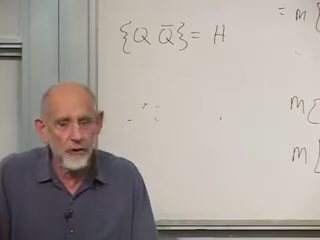
\includegraphics[width=0.62\textwidth]{lecture_05_figure_02.png}\lectureframe{00:55:46.300}\caption{칠판에 나타낸 중심 닫힘 관계. 괄호와 \(Q,\bar Q,H\)가 보이며, 쉼표는 표준 반교환자 표기법에 따라 보충했다.}\end{figure}

진공 에너지는 빈 상태의 에너지가 \(H=0\)가 되도록 정했다. 초대칭 조화진동자에서는 보손과 페르미온의 영점 에너지가 상쇄되므로 이것이 자연스러운 규약이다. \editorialnote{강의에서는 영점 에너지를 따로 표시하지 않고 총 정지 에너지로 직접 계산한다. 여기서 밝힌 규약은 그 선택을 명확히 한다.}

해밀토니안은 짝수다. 또한 대칭 생성자이기도 하다. 시간 병진을 생성하기 때문이다. 따라서 짝수인 시간 병진 생성자를 포함하지 않으면 홀수 생성자만으로 대수가 닫히지 않는다.

\begin{classroomqa}
\audiencequestion{이 관계에서 어떤 항이 짝수인가요? 해밀토니안인가요? \lecturetimestamp{00:58:24}}
\lecturerresponse{그렇다. 에너지는 보통의 관측가능량이므로 \(H\)는 짝수다. 초전하 \(Q\)는 홀수이고, 홀수 양 두 개의 곱은 짝수다. 따라서 \(\{Q,\bar Q\}\)가 \(H\)와 같을 수 있다. 홀수 생성자와 짝수 생성자 사이의 관계는 반교환자가 아니라 교환자로 주어진다.}
\end{classroomqa}

\subsection{대수를 완성하기}

같은 짝홀성의 원소 사이 관계는 자명하다.
\begin{equation}
\{Q,Q\}=2Q^2=0,
\qquad
\{\bar Q,\bar Q\}=2\bar Q^2=0,
\end{equation}
\(Q^2\)에 \(c_-^2\)가 들어 있고 \(\bar Q^2\)에 \(c_+^2\)가 들어 있기 때문이다.

남은 것은 \(H\)와의 관계다. 다음을 두자.
\begin{equation}
H\ket{E}=E\ket{E}.
\end{equation}
보손과 페르미온의 질량이 같으면 \(Q\)는 에너지를 바꾸지 않고 한 입자를 다른 입자로 바꾼다. 따라서 \(Q\ket{E}\)는 0이거나 같은 고유값을 갖는 또 다른 고유상태다.
\begin{equation}
H Q\ket{E}=E Q\ket{E}.
\end{equation}
한편
\begin{equation}
QH\ket{E}=Q(E\ket{E})=E Q\ket{E}.
\end{equation}
두 식을 빼면
\begin{equation}
[H,Q]\ket{E}=0.
\end{equation}
에너지 고유상태들이 완비 기저를 이룬다면, 이는 연산자 항등식으로 성립한다.
\begin{equation}
[H,Q]=0,
\qquad
[H,\bar Q]=0.
\end{equation}

\begin{classroomqa}
\audiencequestion{보손과 페르미온의 질량이 같지 않으면 어떻게 될까요? \lecturetimestamp{01:01:16}}
\lecturerresponse{그러면 한쪽을 다른 쪽으로 바꿀 때 에너지가 변하므로, 제안된 초전하는 해밀토니안과 교환하지 않고 단순한 초대칭은 사라집니다. 구체적으로,
\[
H=m_BN_B+m_FN_F,
\]
명시적인 계산 결과는 다음과 같습니다.
\[
[H,Q]=(m_B-m_F)Q.
\]
이 결과는 \(m_B=m_F\)일 때에만 정확히 0이 됩니다. \editorialnote{질량이 다를 때의 교환자는 에너지 변화 논증을 연산자 형태로 직접 나타내며, 질량이 같아야 한다는 조건을 명시적으로 보여 줍니다.}}
\end{classroomqa}

\begin{classroomqa}
\audiencequestion{에너지 고유상태를 이용한 논증을 좀 더 천천히 다시 설명해 주실 수 있나요? \lecturetimestamp{01:01:37}}
\lecturerresponse{\(H\ket{E}=E\ket{E}\)에서 시작합니다. 질량이 같으면 \(Q\ket{E}\)도 같은 확정 에너지 \(E\)를 가지므로 \(HQ\ket{E}=EQ\ket{E}\)입니다. 반대 순서로 연산하면 \(QH\ket{E}=QE\ket{E}=EQ\ket{E}\)가 됩니다. \(E\)은 보통의 스칼라량이기 때문입니다. 따라서 두 결과의 차이는 모든 에너지 고유상태에서 0입니다. 완비성을 이용하면 이 관계를 각 상태에 대한 명제에서 연산자 방정식 \([H,Q]=0\)으로 확장할 수 있습니다.}
\end{classroomqa}

따라서 모형의 대수 전체는 다음과 같다.
\begin{align}
\{Q,\bar Q\}&=H,\\
\{Q,Q\}&=\{\bar Q,\bar Q\}=0,\\
[H,Q]&=[H,\bar Q]=0.
\end{align}
초전하들은 보존되는 홀수 전하다. 더 놀라운 점은 이들의 대수가 입자 종류를 바꾸는 작용과 시공간 병진 생성자를 결합한다는 것이다.

\section{해밀토니안이 시간 병진을 뜻하는 이유}

이 단순화된 모형에는 공간 좌표는 없지만 시간은 있다. 슈뢰딩거 방정식은 다음과 같다.
\begin{equation}
i\frac{\partial}{\partial t}\ket{\psi(t)}
=H\ket{\psi(t)}.
\end{equation}

\begin{figure}[H]\centering
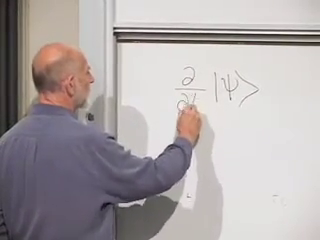
\includegraphics[width=0.56\textwidth]{lecture_05_figure_03.png}\lectureframe{01:07:26.300}\caption{\(\ket{\psi}\)의 시간 미분을 옆에 적고 있다. 손이 분모 일부를 가리고 있지만, 완전한 슈뢰딩거 방정식은 앞에 제시했다.}\end{figure}

유한한 시간 변화 \(\delta\)에 대해
\begin{equation}
\ket{\psi(t+\delta)}
=e^{-iH\delta}\ket{\psi(t)}.
\end{equation}
1차까지 전개하면
\begin{equation}
\ket{\psi(t+\delta)}
=\left(\mathbf 1-i\delta H\right)\ket{\psi(t)}
+O(\delta^2).
\end{equation}
따라서 \(H\)는 시간에 따라 상태를 변화시키는 무한소 생성자다.

아이소스핀이나 색과 같은 내부 대칭도 입자의 표지를 바꾼다. 아이소스핀은 양성자와 중성자 상태를 섞을 수 있고, 색 회전은 빨강, 초록, 파랑 쿼크를 서로 섞는다. 그러나 내부 변환을 아무리 조합해도 계를 공간이나 시간에서 병진시키지는 못한다. 초대칭은 다르다.
\begin{equation}
\begin{gathered}
\text{odd particle-changing transformation}\\
\mathrel{\stackrel{\{\ ,\ \}}{\Longrightarrow}}\\
\text{time translation}
\end{gathered}
\end{equation}
이 점은 홀수 생성자 자체가 보통 좌표와는 다른 좌표를 따른 병진일 수 있음을 시사한다.

\section{초공간}

\subsection{시간과 홀수 좌표의 함수}

다음 함수를 도입하자.
\begin{equation}
\Psi=\Psi(\theta,\bar\theta,t).
\end{equation}
모형에서는 파동함수로, 더 일반적으로는 초장으로 볼 수 있다. 홀수 변수에 대한 전개는 유한 항에서 끝나므로
\begin{equation}
\Psi(\theta,\bar\theta,t)
=A(t)+\bar\chi(t)\theta
+\bar\theta\chi(t)+F(t)\bar\theta\theta.
\end{equation}
하나의 대상에 짝수 성분 함수와 홀수 성분 함수가 함께 들어간다. \editorialnote{이 성분 전개는 앞에서 다룬 그래스만 다항식을 적용한 것이다. 초공간 위의 함수가 구체적으로 어떤 형태인지 표준적인 방식으로 나타낸다.}

보통의 시간 병진은 \(\theta,\bar\theta\)를 고정한 채 다음 변환을 한다.
\begin{equation}
t\longmapsto t+\delta.
\end{equation}
1차까지는
\begin{equation}
\Psi(\theta,\bar\theta,t+\delta)
=\Psi(\theta,\bar\theta,t)
+\delta\,\partial_t\Psi(\theta,\bar\theta,t).
\end{equation}

\begin{figure}[H]\centering
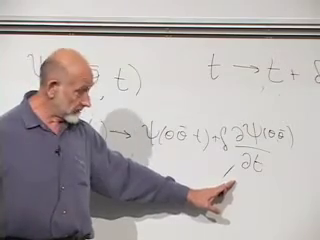
\includegraphics[width=0.72\textwidth]{lecture_05_figure_04.png}\lectureframe{01:13:15.060}\caption{첫 번째 차수에서 \(t\to t+\delta\)를 표시하고 그 아래에 \(\Psi\)의 변화량을 적었다. 미분 항도 바로 옆에 나타나 있다.}\end{figure}

\subsection{홀수 방향의 병진}

이제 홀수 좌표를 이동시키는 변환을 정의하자.
\begin{equation}
\theta\longmapsto\theta+\epsilon,
\end{equation}
여기서 \(\epsilon\)는 또 다른 홀수 그래스만 매개변수다. 이와 함께 시간에도 짝수 멱영 변위를 준다.
\begin{equation}
t\longmapsto t+i\bar\theta\epsilon.
\end{equation}
\(\bar\theta\)와 \(\epsilon\)는 둘 다 홀수이므로 그 곱은 짝수다. 따라서 짝수 좌표 \(t\)에 일관되게 더할 수 있다.

매개변수를 왼쪽으로 옮기면
\begin{equation}
i\bar\theta\epsilon=-i\epsilon\bar\theta.
\end{equation}
유도되는 변화량은 따라서
\begin{align}
\delta_\epsilon\Psi
&=\epsilon\,\partial_\theta\Psi
-i\epsilon\bar\theta\,\partial_t\Psi\\
&=\epsilon q_0\Psi,
\end{align}
이며, 여기서
\begin{equation}
q_0=\partial_\theta-i\bar\theta\partial_t.
\end{equation}
이다. 이 홀수 미분 연산자가 두 변위를 결합한 변환의 생성자다. 왼쪽 미분을 사용할 때 이에 맞는 켤레 생성자는 다음과 같다.
\begin{equation}
\bar q_0=-\partial_{\bar\theta}
+i\theta\partial_t.
\end{equation}

정확한 부호는 왼쪽 그래스만 미분과 오른쪽 그래스만 미분 중 어느 것을 사용하는지, 그리고 켤레화할 때 홀수 인자의 순서를 어떻게 뒤집는지에 따라 달라집니다. 어떤 규약을 사용하더라도 시간 병진으로의 닫힘은 변하지 않아야 합니다. 위에서 정의한 것을 사용하면,
\begin{align}
\{q_0,\bar q_0\}
&=i\{\partial_\theta,\theta\}\partial_t
+i\{\bar\theta,\partial_{\bar\theta}\}\partial_t\\
&=2i\partial_t.
\end{align}
미분 연산자끼리의 항은 사라지고 홀수 좌표에 대한 이차항도 사라집니다. 두 혼합항은 각각 \(i\partial_t\)를 줍니다.

슈뢰딩거 그림의 상태에서는 \(H=i\partial_t\)이므로
\begin{equation}
\{q_0,\bar q_0\}=2H.
\end{equation}
다음과 같이 정규화하면
\begin{equation}
q=\frac{q_0}{\sqrt2},
\qquad
\bar q=\frac{\bar q_0}{\sqrt2},
\end{equation}
다음을 얻는다.
\begin{equation}
\boxed{\{q,\bar q\}=H.}
\end{equation}
\editorialnote{강의에서는 부호가 확실하지 않은 상태로 계산을 진행한 뒤 계수 2가 생김을 확인한다. 위의 왼쪽 미분 규약은 강의의 계산을 유지하면서 일관된 정규화를 하나 정해 준다. 다른 표준 규약을 쓰면 부호가 좌표 변위와 생성자 사이에서 옮겨간다.}

\begin{classroomqa}
\audiencequestion{초공간 반교환자에 마지막 계수 2가 나타나는 이유는 무엇인가요? \lecturetimestamp{01:24:21}}
\lecturerresponse{같은 혼합 항이 두 개 있기 때문이다. 하나는 \(\{\partial_\theta,\theta\}=1\)에서, 다른 하나는 \(\{\partial_{\bar\theta},\bar\theta\}=1\)에서 나온다. 둘 다 시간 미분 항을 곱한다. 따라서 정규화하지 않은 생성자는 \(2i\partial_t\)를 주며, 각 초전하에 계수 \(1/\sqrt2\)를 곱하면 앞서 쓴 정규화가 복원된다.}
\end{classroomqa}

\begin{classroomqa}
\audiencequestion{\(\epsilon\)가 작다는 가정을 사용해 이 구성을 만들었나요? \lecturetimestamp{01:24:51}}
\lecturerresponse{보통의 수치적 크기가 아니라 멱영성을 이용했다. \(\epsilon^2=0\)이므로 \(\epsilon\)에 대한 모든 전개는 1차 항 뒤에서 끝난다. 무한소나 작은 양이라고 부르는 것은 유용한 비유지만, 전개가 끝나는 것은 정확한 결과다.}
\end{classroomqa}

\editorialnote{그래스만 매개변수에는 보통의 양의 크기가 없다. 이들이 무한소 매개변수 역할을 하는 까닭은 멱영성과 전개의 정확한 종료에 있다.}

\subsection{기하학적 의미}

이제 대수를 구현하는 서로 동등한 두 방식이 있다. 조화진동자 관점에서는 \(Q\)와 \(\bar Q\)가 페르미온을 보손으로, 보손을 페르미온으로 바꾼다. 기하학적 관점에서는 \(q\)와 \(\bar q\)가 홀수 방향으로 함수를 병진시키면서 보통의 시간 변위도 일으킨다. 두 관점 모두에서
\begin{equation}
\begin{gathered}
\{\text{supercharge},\text{conjugate supercharge}\}\\
=\text{time-translation generator}.
\end{gathered}
\end{equation}

\(t,\theta,\bar\theta\)를 포함하는 일반화된 좌표 공간이 초공간이다. 상대론적 장 이론에서는 여기에 보통의 공간 좌표도 포함되며, 초전하들은 \(H=P_0\)뿐 아니라 전체 시공간 운동량 \(P_\mu\)으로 닫힌다. 이 구조를 곡률이 있는 공간으로 확장하면 초중력으로 이어진다.

한편으로 그래스만 변수는 보손과 페르미온을 효율적으로 추적하는 도구다. 다른 한편으로 닫힘 관계는 훨씬 더 깊은 것을 말해 준다. 입자의 종류와 시공간 기하 사이의 구분은 더 이상 절대적이지 않다. 홀수 방향으로 두 번 이동하면 보통의 방향으로 움직이게 된다. 자연이 이 구조를 실험적으로 구현하는지는 별개의 문제다. 이 구조가 일관되고 간결하며 놀라울 만큼 엄격한 수학적 틀이라는 사실은 변하지 않는다.
